\section{Resultados y Discusión} \label{sec:resultados}

Los resultados obtenidos durante la experimentación se han almacenado en una base de datos DuckDB, tal y como se describió en la Sección \ref{sec:infraestructura_exp}. Las tablas generadas contienen, para cada ejecución realizada, tanto los metadatos asociados al entrenamiento como las métricas obtenidas durante su evaluación.

Con el objetivo de reducir la influencia de posibles valores atípicos (\textit{outliers}) sobre el análisis estadístico, se han creado vistas derivadas de cada tabla en las que se eliminan aquellos registros cuyos valores de \textit{accuracy} se encuentran fuera de un intervalo de tres desviaciones estándar respecto a la media. Este procedimiento, basado en el método \textit{Z-Score} \cite{venkataanusha_DetectingOutliers2019}, se define como:

\[
z = \frac{x - \mu}{\sigma}
\]

donde \(x\) representa el valor analizado, \(\mu\) la media de la distribución y \(\sigma\) la desviación estándar. De esta forma, se consideran valores atípicos aquellos que cumplen:

\[
|z| > 3
\]

Además, también se han eliminado aquellos registros correspondientes a entrenamientos incompletos o interrumpidos, con el fin de garantizar la consistencia de los resultados analizados.

Tras aplicar este proceso de filtrado, el número total de registros válidos quedó reducido de la siguiente manera:

\begin{itemize}
    \item Tabla de entrenamientos: de 1917 registros originales se eliminaron 105, obteniéndose un total de 1812 registros válidos.
    
    \item Tabla de trials: de 5751 registros originales se eliminaron 515, obteniéndose un total de 5246 registros válidos.
    
    \item Tabla de clases: de 15336 registros originales se eliminaron 3331, obteniéndose un total de 12605 registros válidos.
\end{itemize}

En esta sección se presentarán estos resultados, los cuales se discutirán y analizarán siguiendo la siguiente metodología:

Primero se analizarán los resultados obtenidos por cada modelo en función de la tarea 

\subsection{Tarea Estática} \label{sec:tareaestatica} 

\subsubsection{Comparación de Global}

\begin{figure}[H]
    \centering
    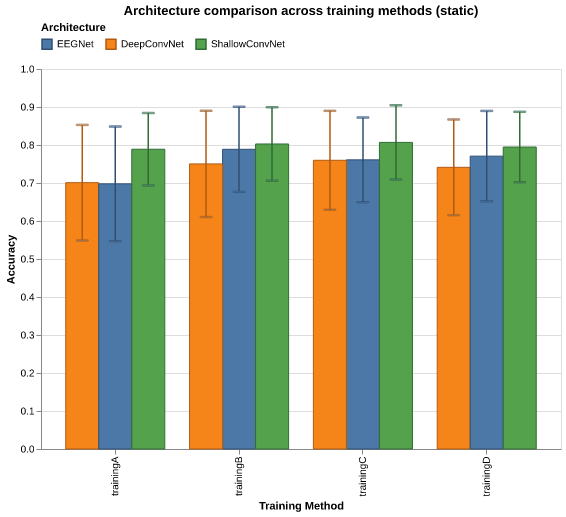
\includegraphics[width=0.90\textwidth]{img/resultados/architecture_training_comparison_clean_static.png}
    %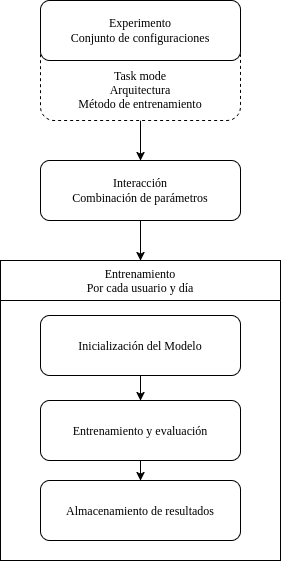
\includegraphics[height=\dimexpr\pagegoal-\pagetotal-\baselineskip\relax,width=\textwidth,keepaspectratio]{img/diagrama_pipeline.drawio.png}
    \caption{Comparación general de las distintas arquitecturas y métodos de entrenamiento en la tarea estática}
    \label{fig:architecture_training_comparison_clean_static}
\end{figure}


Me da igual todo, solo me centro en los modelos. hago avg y std con los metodos y los usuarios 

\subsubsection{Comparación de Método de Entrenamiento}
Me da igual todo, solo me centro en los metodos. hago avg y std con los modelos y los usuarios 

\subsubsection{Variabilidad Entre Usuarios}

\begin{figure}[H]
    \centering
    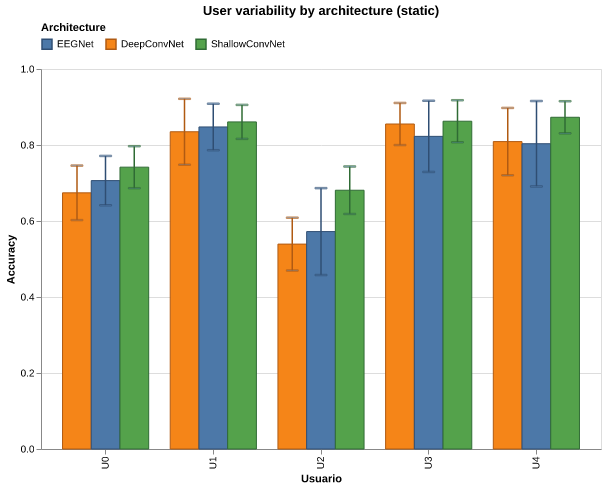
\includegraphics[width=0.90\textwidth]{img/resultados/user_variability_by_model_static.png}
    %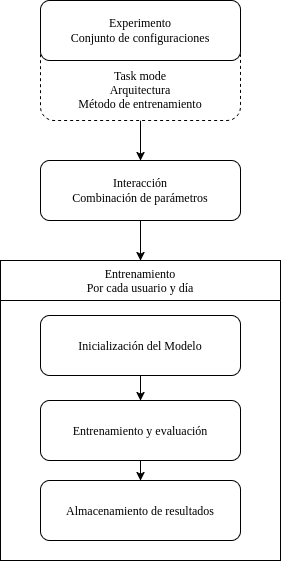
\includegraphics[height=\dimexpr\pagegoal-\pagetotal-\baselineskip\relax,width=\textwidth,keepaspectratio]{img/diagrama_pipeline.drawio.png}
    \caption{Variabilidad entre usuarios en la tarea estática}
    \label{fig:user_variability_by_model_static}
\end{figure}

\subsubsection{Mejor Configuración}

\begin{figure}[H]
    \centering
    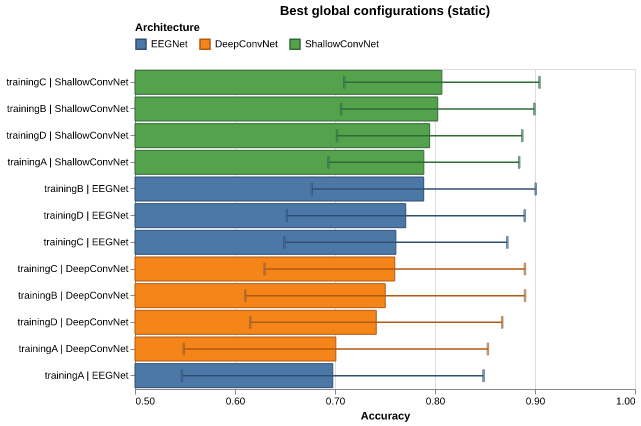
\includegraphics[width=1\textwidth]{img/resultados/best_global_configurations_static.png}
    %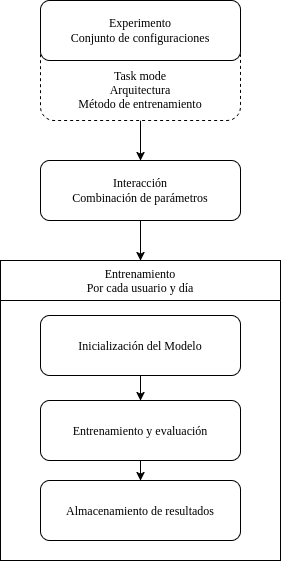
\includegraphics[height=\dimexpr\pagegoal-\pagetotal-\baselineskip\relax,width=\textwidth,keepaspectratio]{img/diagrama_pipeline.drawio.png}
    \caption{Mejores configuraciones globales en la tarea estática}
    \label{fig:best_global_configurations_static}
\end{figure}

\subsection{Tarea Movimiento} \label{sec:tareamovimiento} 
mismo esquema 

\subsubsection{Comparación de Global}

\begin{figure}[H]
    \centering
    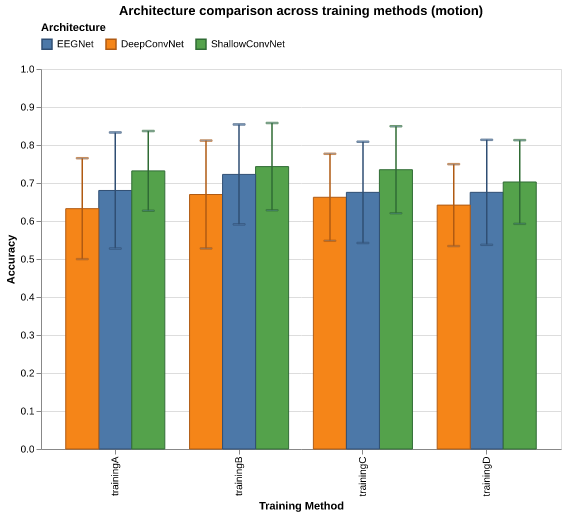
\includegraphics[width=0.90\textwidth]{img/resultados/architecture_training_comparison_clean_motion.png}
    %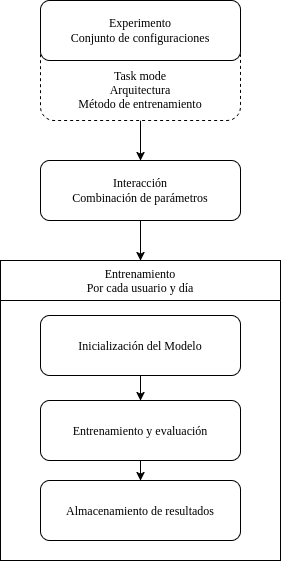
\includegraphics[height=\dimexpr\pagegoal-\pagetotal-\baselineskip\relax,width=\textwidth,keepaspectratio]{img/diagrama_pipeline.drawio.png}
    \caption{Comparación general de las distintas arquitecturas y métodos de entrenamiento en la tarea de movimiento}
    \label{fig:architecture_training_comparison_clean_motion}
\end{figure}


\subsubsection{Comparación de Método de Entrenamiento}
\subsubsection{Variabilidad Entre Usuarios}
\begin{figure}[H]
    \centering
    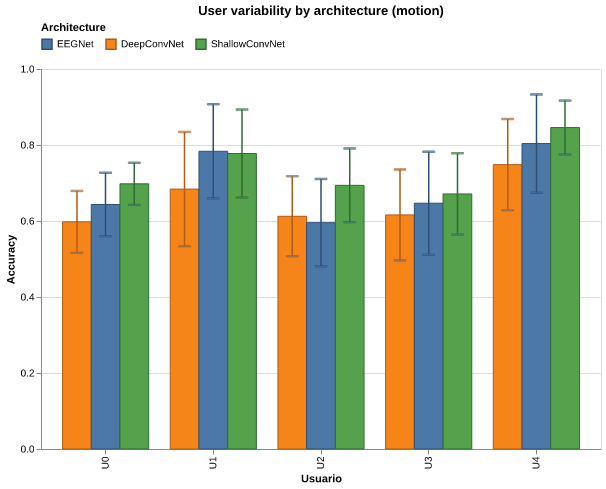
\includegraphics[width=0.90\textwidth]{img/resultados/user_variability_by_model_motion.png}
    %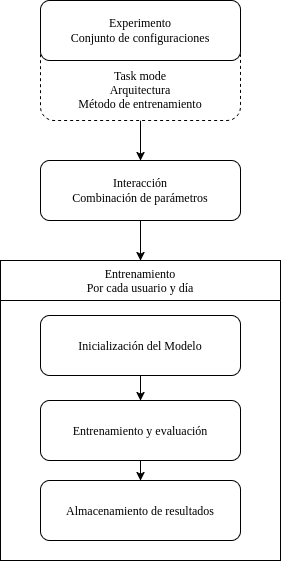
\includegraphics[height=\dimexpr\pagegoal-\pagetotal-\baselineskip\relax,width=\textwidth,keepaspectratio]{img/diagrama_pipeline.drawio.png}
    \caption{Variabilidad entre usuarios en la tarea de movimiento}
    \label{fig:user_variability_by_model_motion}
\end{figure}

\subsubsection{Mejor Configuración}

\begin{figure}[H]
    \centering
    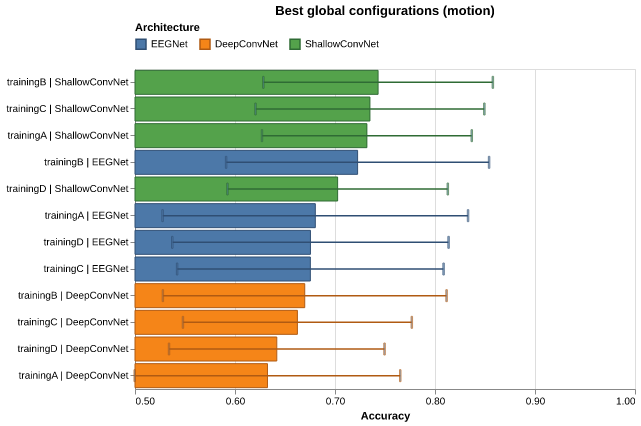
\includegraphics[width=1\textwidth]{img/resultados/best_global_configurations_motion.png}
    %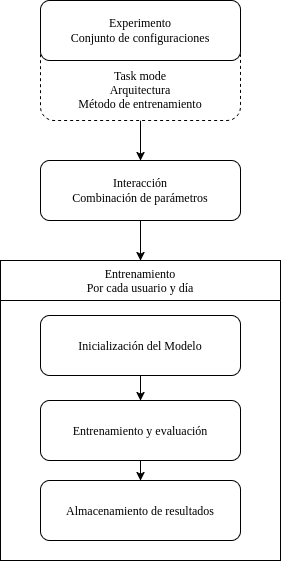
\includegraphics[height=\dimexpr\pagegoal-\pagetotal-\baselineskip\relax,width=\textwidth,keepaspectratio]{img/diagrama_pipeline.drawio.png}
    \caption{Mejores configuraciones globales en la tarea de movimiento}
    \label{fig:best_global_configurations_motion}
\end{figure}

\subsection{Comparación entre tareas}


\begin{figure}[H]
    \centering
    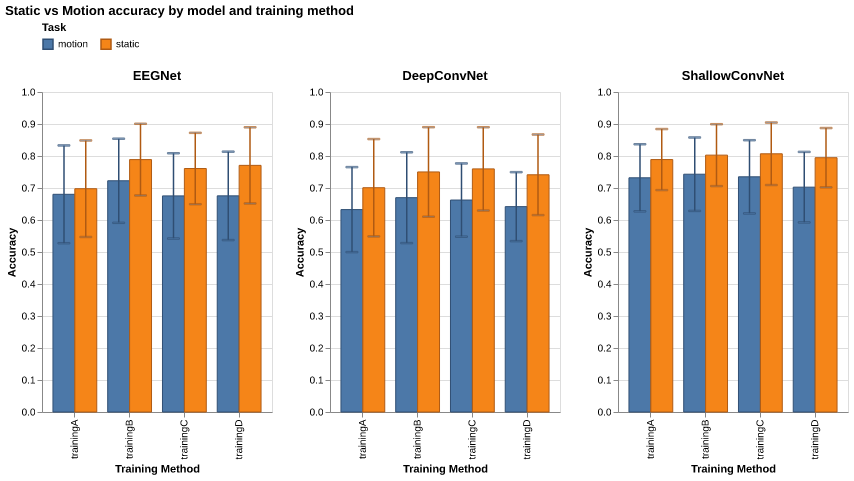
\includegraphics[width=1\textwidth]{img/resultados/static_vs_motion_accuracy.png}
    %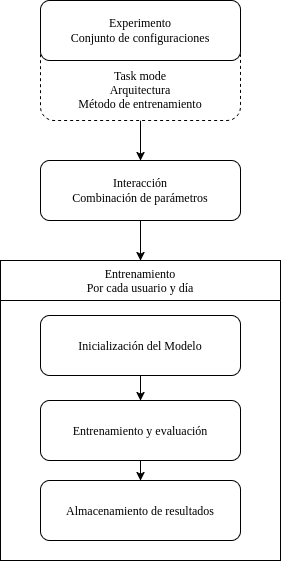
\includegraphics[height=\dimexpr\pagegoal-\pagetotal-\baselineskip\relax,width=\textwidth,keepaspectratio]{img/diagrama_pipeline.drawio.png}
    \caption{Comparación de la precisión entre la tarea estática y la de movimiento}
    \label{fig:static_vs_motion_accuracy}
\end{figure}

